\documentclass{deltares_memo}
\usepackage{CJKutf8}
\newcommand{\menuarrow}{$\rightarrow$}
\newcommand{\plotcfts}{PlotCFTS\xspace}
\newcommand{\dflowfm}{D-Flow FM\xspace}
\newcommand{\qumesh}{QGIS\_UMESH\xspace}
\newcommand{\netcdf}{netCDF\xspace}
\newcommand{\cfstandard}{Climate and Forecast 1.7 standard\xspace}

\begin{document}
\memoTo{To whom it may concern}
\memoConfidentialUntil{}
\memoDate{\today}
\memoVersion{001}
\memoFrom{Jan Mooiman}
\memoTelephone{---}
\memoEmail{jan.mooiman@deltares nl}
\memoSubject{Manual to plot result files of \dflowfm in QGIS 3.12 (map- and history-files)}
\memoCopy{}

\deltarestitle

\tableofcontents

%--------------------------------------------------------------------------------
\section{Release Notes}
\phantom{m}\vspace{-\baselineskip}
%
%--- begin light blue table ---
\begin{longtable}{p{16mm-12pt}|p{\textwidth-16mm-12pt}} 
%\caption{Light blue theme of table} \\% 
\rowcolor{dblue1} 
\textbf{Release} 
& \textbf{Description} 
\\ 
\topline 
\endfirsthead 
\endhead 
\endfoot 
\bottomline 
\endlastfoot 
0.00.00  &  - No information available.  \\
\end{longtable} 
%--- end light blue table ---
%
%--------------------------------------------------------------------------------
\section{Menu bar}
\phantom{m}\vspace{-\baselineskip}
\begin{figure}[H]
    \centering    
    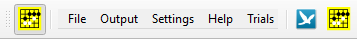
\includegraphics[width=0.40\textwidth]{pictures/menu_bar.png}
    \caption{The menu bar of the \qumesh plugin}
\end{figure}

%------------------------------------------------------------------------------
\subsection{File}
\phantom{m}\vspace{-\baselineskip}
\begin{figure}[H]
    \centering    
    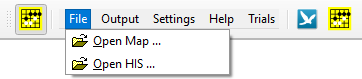
\includegraphics[width=0.40\textwidth]{pictures/menu_file.png}
    \caption{Menu \menuarrow File}
\end{figure}

%--------------------------------------------------------------------------------
\subsubsection{Open UGRID}
When selecting this option you are able to select \netcdf files which are meet the UGRID standard. 
Example files are the mesh- and map-file of the \dflowfm program (\file{$\ast$\_net.nc}, \file{$\ast$\_map.nc}).
Only the map-file could contain time series.
%--------------------------------------------------------------------------------
\subsubsection{Open HisCF}
When selecting this option you are able to select \netcdf files which are meet the climate and forecast history file standard.
Example files are the history output files of the program \dflowfm (\file{$\ast$\_his.nc}).
%--------------------------------------------------------------------------------
\subsection{Output}
\phantom{m}\vspace{-\baselineskip}
\begin{figure}[H]
    \centering    
    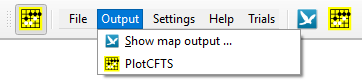
\includegraphics[width=0.40\textwidth]{pictures/menu_output.png}
    \caption{Menu \menuarrow Output}
\end{figure}

%------------------------------------------------------------------------------
\subsubsection{Show map output}
After selecting \menu{Output\menuarrow Show map output} the window \window{Map Output Animation} will open, see as example \autoref{fig:map_output_a}.
\begin{figure}[H]
\begin{subfigure}[b]{0.48\textwidth}
	\centering    
	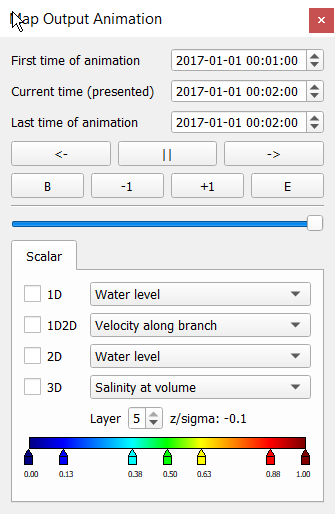
\includegraphics[width=\textwidth]{pictures/map_output_animation_window_scalar.png}
	\caption{Layout scalar quantities\label{fig:map_output_a}}
\end{subfigure}
\hfill
\begin{subfigure}[b]{0.48\textwidth}
	\centering    
	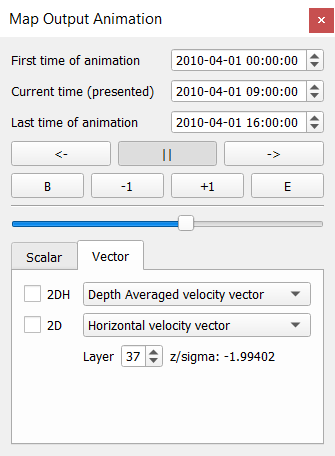
\includegraphics[width=\textwidth]{pictures/map_output_animation_window_vector.png}
	\caption{Layout vector quantities}
\end{subfigure}    
    \caption{\window{Map Output Animation} window for scalars and vector.}
\end{figure}

%------------------------------------------------------------------------------
\subsubsection{PlotCFTS}
After selecting \menu{Output\menuarrow \plotcfts} the program \plotcfts will start, see as example \autoref{fig:plotcfts_main}.
Select from the menubar of the \plotcfts program menu option \menu{Help \menuarrow User Manual} to open the user manual for the program \plotcfts. 

\begin{figure}[H]
    \centering    
    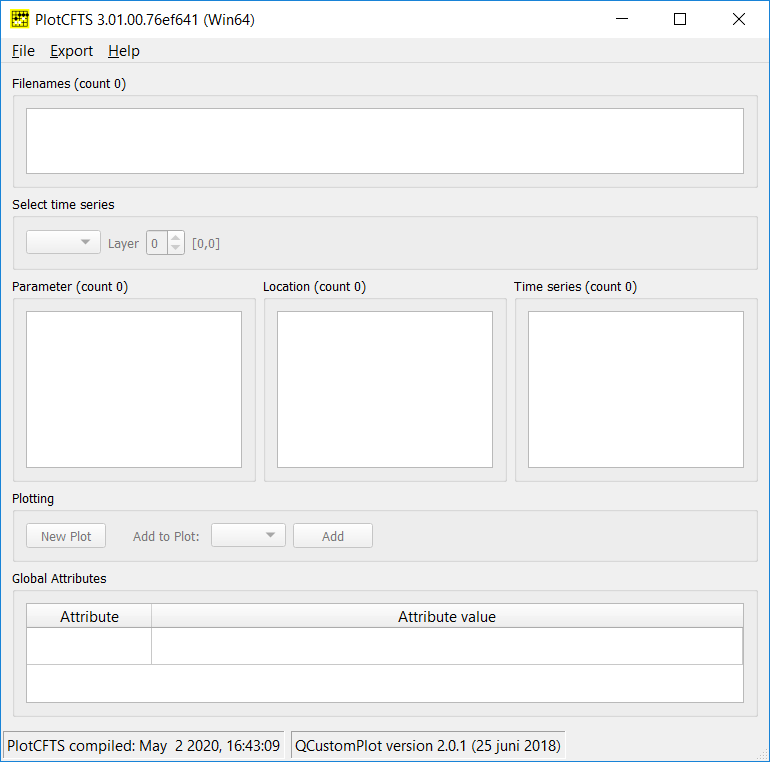
\includegraphics[width=0.9\textwidth]{pictures/main_plotcfts.png}
    \caption{Main window of the \plotcfts program.\label{fig:plotcfts_main}}
\end{figure}
%--------------------------------------------------------------------------------
\subsection{Settings}
Settings for the presentation of scalars and vectors.
\begin{figure}[H]
    \centering    
    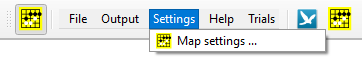
\includegraphics[width=0.40\textwidth]{pictures/menu_settings.png}
    \caption{Menu \menuarrow Settings}
\end{figure}
When selecting this option some settings for the presentation of the variables via the window \window{Map Output Animation} can be set. 
This window will also pop up when using the right mouse button within the window \window{Map Output Animation}.
\begin{figure}[H]
	\centering    
	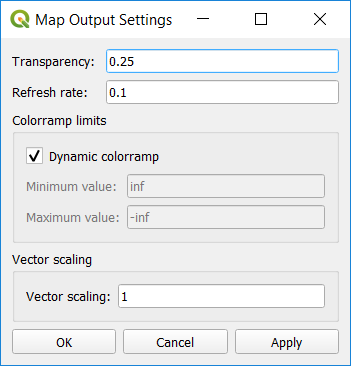
\includegraphics[width=0.40\textwidth]{pictures/map_properties.png}
	\caption{Menu \menuarrow Settings}
\end{figure}
where
\begin{longtable}{p{35mm-12pt} p{\textwidth-35mm-12pt}} 
	Transparency & Specify the transparency of the iso patches for the scalars. \\
	\textbf{Colorramp limits} & \\
	Dynamic colorramp\newline (\textit{checked}) & Colorramp limits are determined by the minimum and maximum value of the scalar. 
	These values reach their extreme values after all timestep are visualised.\\
	Dynamic colorramp\newline (\textit{unchecked}) & \\
	Minimum value & specify the minimum value for the scalar.\\
	Maximum value & specify the maximum value for the scalar.\\
	\textbf{Vector scaling} & \\
	Vector scaling & The vector of length 1 (ex.\ \SI{1}{\metre\per\second}) is scaled with this factor. The drawing length is based on the averaged cell size.
\end{longtable}
%--------------------------------------------------------------------------------
\subsection{Help}
\phantom{m}\vspace{-\baselineskip}
\begin{figure}[H]
    \centering    
    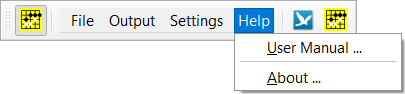
\includegraphics[width=0.4\textwidth]{pictures/menu_help.png}
    \caption{Menu \menuarrow Help}
\end{figure}

%--------------------------------------------------------------------------------
\subsubsection{User Manual}
Shows the user manual
\begin{figure}[H]
	\centering    
	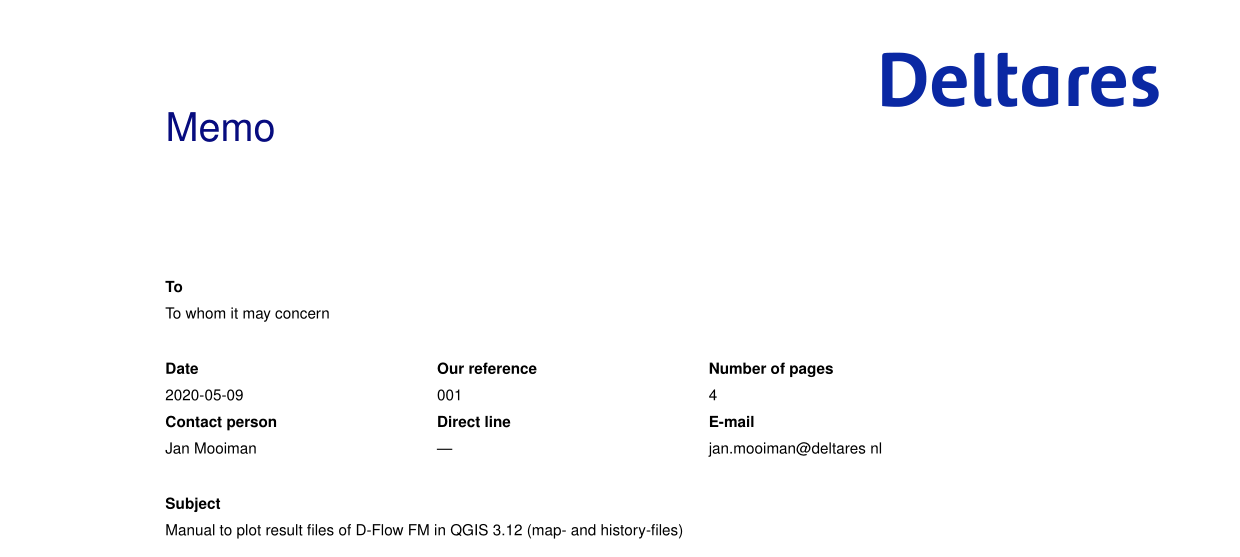
\includegraphics[width=0.9\textwidth]{pictures/menu_help_user_manual.png}
	\caption{\qumesh user manual}
\end{figure}

%--------------------------------------------------------------------------------
\subsubsection{About}
Shows the about box.
\begin{figure}[H]
    \centering    
    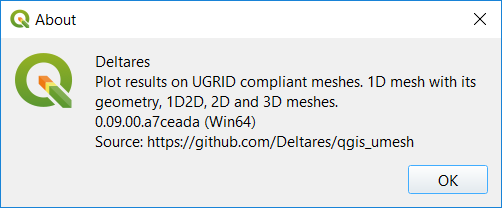
\includegraphics[width=0.4\textwidth]{pictures/menu_help_about.png}
    \caption{About box}
\end{figure}
%--------------------------------------------------------------------------------
%\subsection{Trials}
%\phantom{m}\vspace{-\baselineskip}
%\begin{figure}[H]
%    \centering    
%    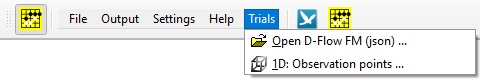
\includegraphics[width=0.40\textwidth]{pictures/menu_trials.png}
%    \caption{Menu \menuarrow Trials}
%\end{figure}
%------------------------------------------------------------------------------
\section{Source}
The source code is available on GitHUB:
\begin{Verbatim}
https://github.com/Deltares/qgis_umesh
\end{Verbatim}
%------------------------------------------------------------------------------

\end{document}
